\documentclass{beamer}
\usepackage[latin1]{inputenc}

\usepackage[brazil]{babel}

%\documentclass[ucs]{beamer}%para sistemas com ucs
%\usepackage[utf8x]{inputenc}%idem
\usetheme{Frankfurt} %apenas um dos muitos temas dispon�veis: Antibes, Bergen, Berkeley, default, Darmstadt, Boadila, Madrid, Pittsburgh, Rochester, Copenhagen, Warsaw, Singapore, Malmoe, Dresden, Frankfurt, Goettingen, Hannover, Ilmenau, JuanLesPins, Luebeck, Marburg, Montpellier, PaloAlto, Szeged, boxes
\usepackage{algorithm}
\usepackage{algorithmic}
 
\title[Extra\c{c}\~ao de Informa\c{c}\~ao na Web]{Trabalho de Conclus\~ao de Curso \\ Extra\c{c}\~ao de Informa\c{c}\~ao na Web}
\author[Mario H. Adaniya]{Aluno: M\'ario Henrique Akihiko da Costa Adaniya \\Orientador: Prof. Dr. Mario Lemes Proen�a Jr.}
\institute{\large Universidade Estadual de Londrina}
\date{\today}
\logo{
\includegraphics[scale=0.15]{./figuras/uellogo1.jpg}}

\begin{document} 
  
%	\AtBeginSection[] 
%	{
%		\begin{frame}
%		\frametitle{Sum�rio} 
%		\tableofcontents[currentsection]
%		\end{frame}
%	}
 
%para criar a p�gina de rosto
	\frame{\titlepage} %inclui a front page 
%==================================================slide
% cria o sum�rio
	\begin{frame}
	 \frametitle{Sum�rio}
	 \tableofcontents%[pausesections]
	\end{frame}
%-----------------------------------------------------
%==================================================slide
%criando um slide
	\section{Introdu\c{c}\~ao}
	\begin{frame}
	\frametitle{Introdu\c{c}\~ao}
		\begin{itemize}
			\item Sistema de Computa\c{c}\~ao Paralela: conjunto de processadores interconectados conforme alguma topologia para permitir controle de suas atividades e troca de dados \cite{CACERES2001};
			\item Processamento Paralelo: \'e uma forma eficiente de processar informa\c{c}\~ao a qual enfatiza a explora\c{c}\~ao de eventos concorrentes na computa\c{c}\~ao do processo \cite{DIVERIO2002}.
		\end{itemize}
	\end{frame}

	\begin{frame}
	\frametitle{Introdu\c{c}\~ao}
		\begin{itemize}
			\item Utilizado onde grande demanda de poder computacional \'e exigida:
				\begin{itemize}
					\item Previs\~oes metereol\'ogicas;
					\item Simula\c{c}\~oes de engenharia;
					\item Resolu\c{c}\~ao de Sistemas Lineares de grande porte.
				\end{itemize}
			\item M\'aquinas paralelas:
			\begin{itemize}
				\item Alto custo; 
			 	\item Exemplos: Cray-1, Cray X-MP;
			\end{itemize}

			\item Clusters Beowulf (1994): equipamentos de prateleira e {\it software} livre.
		\end{itemize}
	\end{frame}

	\begin{frame}
	\frametitle{Introdu\c{c}\~ao}
		\begin{itemize}
			\item Objetivos deste trabalho:
				\begin{itemize}
					\item Realizar estudo sobre arquiteturas paralelas;
					\item Apresentar modelos para a constru\c{c}\~ao de algoritmos paralelos;
					\item Construir e utilizar ambientes paralelos;
					\item Apresentar a paraleliza\c{c}\~ao de um algoritmo de treinamento de uma Rede Neural Artificial.
				\end{itemize}
		\end{itemize}
	\end{frame}

	\section{Recupera\c{c}\~ao de Informa\c{c}\~ao}

	\begin{frame}
		\frametitle{\huge Recupera\c{c}\~ao de Informa\c{c}\~ao}
		\Large		
		\begin{block}{\Large O que \'e?}
			\justifying
			Recupera\c{c}\~ao de Informa\c{c}\~ao (RI) \'e a tarefa de encontrar documentos relevantes a partir de um \textit{corpus} ou conjunto de textos em resposta a uma necessidade de informa\c{c}\~ao de um usu\'ario.% \cite{Smeaton1997}.		
		\end{block}
	\end{frame}
	

	\begin{frame}
	\Large
		\frametitle{\huge Recupera\c{c}\~ao de Informa\c{c}\~ao}
		\framesubtitle{\Large Cl\'assica}		
			\begin{itemize}
			  	\justifying 
				\item \textbf{Entrada}: Cole\c{c}\~ao de documentos + Query do usu\'ario
				\item Objetivo: Recuperar documentos ou textos com informa\c{c}\~ao relevantes ao usu\'ario
	
				\item Dois Aspectos:
					\begin{itemize}
					 	\item Processamento da cole��o de documentos;
						\item Processamento de consultas (pesquisa);
					\end{itemize} 
			\end{itemize}
	\end{frame}

	\begin{frame}
		\frametitle{\huge Recupera\c{c}\~ao de Informa\c{c}\~ao}
		\framesubtitle{\Large Cl\'assica}
		\LARGE
			\begin{itemize}
			 	\item Modelo L�gico:
					\begin{itemize}
					 	\item AND, OR, NOT.
					\end{itemize}
			 	\item Modelo L�gico:
					\begin{itemize}
					 	\item + grau de compara��o;
					 	\item fun��o de ordena��o;
					\end{itemize}
			 	\item Modelo L�gico:
					\begin{itemize}
					 	\item Documentos e query representada por vetor de termos;
					\end{itemize}
			 	\item Modelo PLN:
					\begin{itemize}
					 	\item Estrutura e significado ligados;
					\end{itemize}
			\end{itemize}
	\end{frame}
	
	\begin{frame}	
		\frametitle{\huge Recupera\c{c}\~ao de Informa\c{c}\~ao}
		\framesubtitle{\Large Na Web}
		\Large		
			\begin{itemize}
			  \justifying 
				\item Entrada: Web + Query do usu\'ario
				\item Objetivo: Recuperar p\'aginas de alta qualidade com conte\'udos relevantes para o usu\'ario
					\begin{itemize}
					 	\item Est\'atico (texto, \'audio, v\'ideo,\ldots)
						\item Din\^amico
					\end{itemize}
				\item Dois Aspectos:
					\begin{itemize}
					 	\item Processamento e representar a cole\c{c}\~ao de documentos;
							\begin{itemize}
							 	\item Agrupando as p\'aginas est\'aticas
								\item ``Aprender'' sobre p\'aginas din\^amicas
							\end{itemize}
						\item Processamento de consultas (pesquisa);
					\end{itemize}
			\end{itemize}
	\end{frame}
		
	\begin{frame}	
		\frametitle{\huge Recupera\c{c}\~ao de Informa\c{c}\~ao}
		\framesubtitle{\Large Caracter\'isticas da Web}
		\large		
			\begin{itemize}
			  \justifying 
				\item Tamanho da Internet
				\item Duplica��o - 30\% do conte\'udo \'e c\'opia de algum conte\'udo existente	
				\item Heterogenidade:
					\begin{itemize}
					 	\item Tipos de documentos - texto, figuras, scripts,\ldots;
						\item Qualidade - Desde textos em blogs at\'e artigos cient\'ificos
						\item Idiomas - 100+
					\end{itemize}
				\item M\'ultiplos usu\'arios - cada um utiliza a Internet de uma maneira
				\item Alta Linkagem (High Linkage) - Cada p\'agina cont\'em aproximadamente 8 links para outras p\'aginas
			\end{itemize}
	\end{frame}
	\section{Extra\c{c}\~ao de Informa\c{c}\~ao}
	\begin{frame}
		\frametitle{\huge Extra\c{c}\~ao de Informa\c{c}\~ao}
		\begin{block}{\Large O que �?}
			\begin{itemize}
				\item A tarefa de identificar os fragmentos espec\'ificos de um \'unico documento que constituem o seu n\'ucleo sem\^antico
				\begin{itemize}
					\item Ex.: Relat\'orio de Clima e Tempo \Rightarrow  datas, temperaturas, locais.
				\end{itemize}
			\end{itemize}
		\end{block}		

	\end{frame}
	
	\begin{frame}
		\frametitle{MUC - Message Understanding Conference}			
		\begin{table}[htbp]
		  %\caption{Confer�ncias e seus temas}
		  \centering
		  \footnotesize
		  %\scriptsize
		  %\tiny
		    \begin{tabular}{cccc}
			    \addlinespace
			    \toprule
			    {\bf Confer�ncia} & {\bf Ano} & {\bf Fonte de Texto} & {\bf T�pico(Dominio)} \\
			    \midrule
			    MUC-1 & 1987 & Artigos Militares & Opera��es de fuga\\
			    MUC-2 & 1989 & Artigos Militares & Opera��es de fuga\\
			    MUC-3 & 1991 & Artigos de Jornais & Atividades Terroristas \\% na Am�rica Latina \\
			    MUC-4 & 1992 & Artigos de Jornais & Atividades Terroristas \\ %na Am�rica Latina \\
			    MUC-5 & 1993 & Artigos de Jornais & Corporate Joint Ventures\\
			    MUC-6 & 1995 & Artigos de Jornais & Negotiation of Labor Disputes \\
			    MUC-7 & 1997 & Artigos de Jornais & Acidente de avi�es \\
			    \bottomrule
		    \end{tabular}
		  \label{tab:MUC}
		\end{table}
		
	\end{frame}
	
	\begin{frame}
		\frametitle{\huge Tipos de Dados}
		\framesubtitle{\Large Documentos Livre}
			\begin{figure}[htb]
				\begin{center}				
					
\includegraphics[scale=0.5]{./figuras/texto.png}				
				\end{center}
			\end{figure}		
	\end{frame}
	
	\begin{frame}
		\frametitle{\huge Tipos de Dados}
		\framesubtitle{\Large Documentos Semi-Estruturado}
			\begin{figure}[htb]
				\begin{center}				
					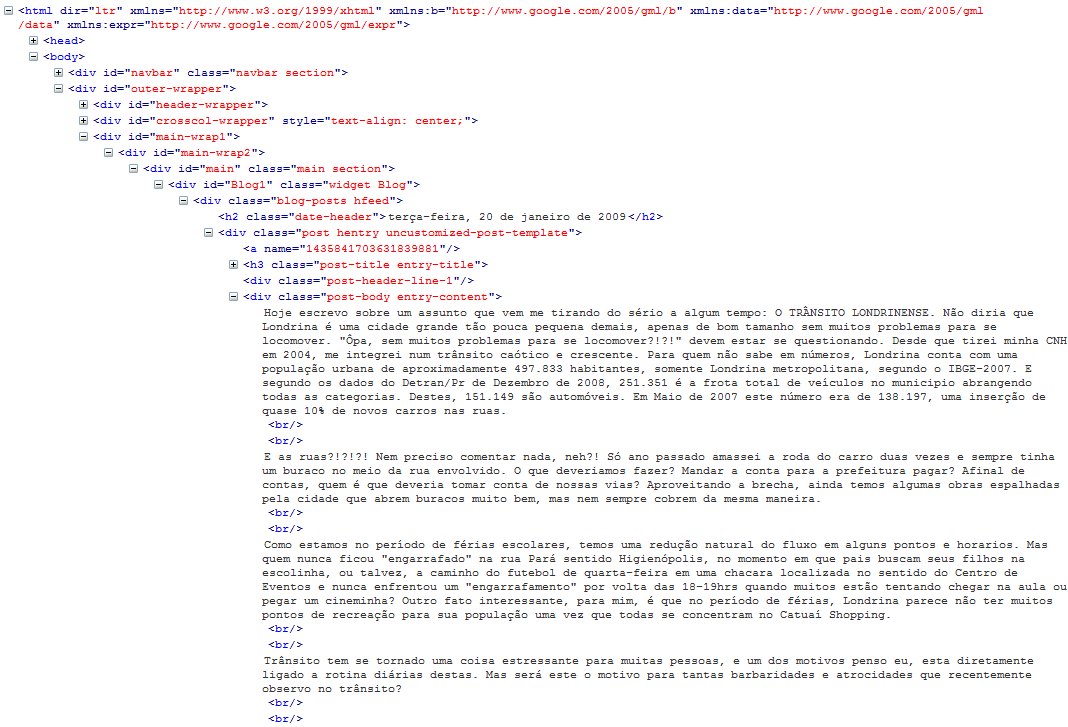
\includegraphics[scale=0.5]{./figuras/html.png}				
				\end{center}
			\end{figure}
	\end{frame}
	
	\begin{frame}
		\frametitle{\huge Tipos de Dados}
		\framesubtitle{\Large Documentos Estruturado}
			\begin{figure}[htb]
				\begin{center}				
					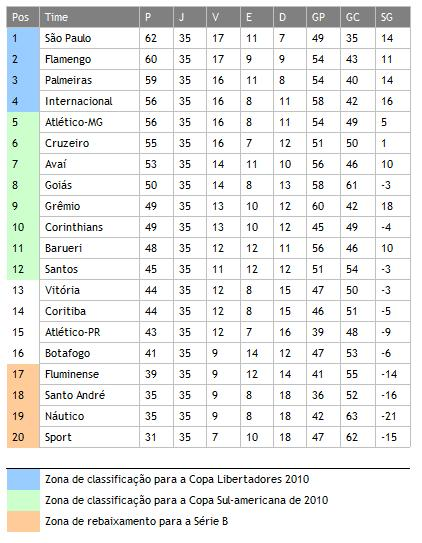
\includegraphics[scale=0.6]{./figuras/tabela.jpg}
				\end{center}
			\end{figure}		
	\end{frame} 
	
	\begin{frame}
		\frametitle{\huge Extra\c{c}\~ao de Informa\c{c}\~ao}	
		\framesubtitle{\Large FLUXO GERAL}			
			\begin{figure}[htb]
				\begin{center}				
					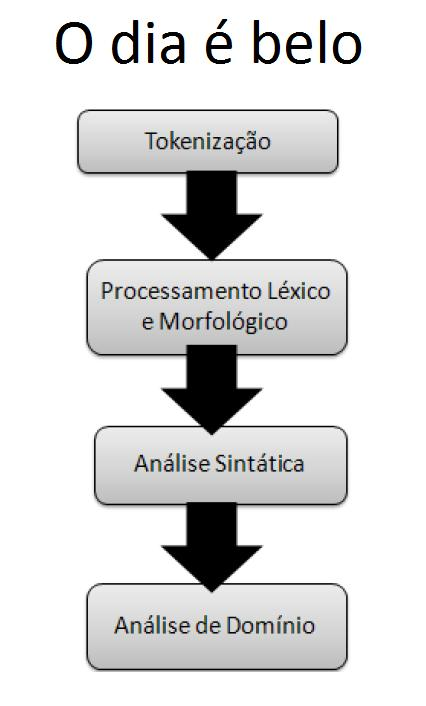
\includegraphics[scale=0.3]{./figuras/processo00.jpg}				
				\end{center}				
			\end{figure}
	\end{frame}

	\begin{frame}
		\frametitle{\huge Extra\c{c}\~ao de Informa\c{c}\~ao}	
		\framesubtitle{\Large AVALIA\c{C}\~AO}		
			\begin{figure}[htb]
				\begin{center}				
					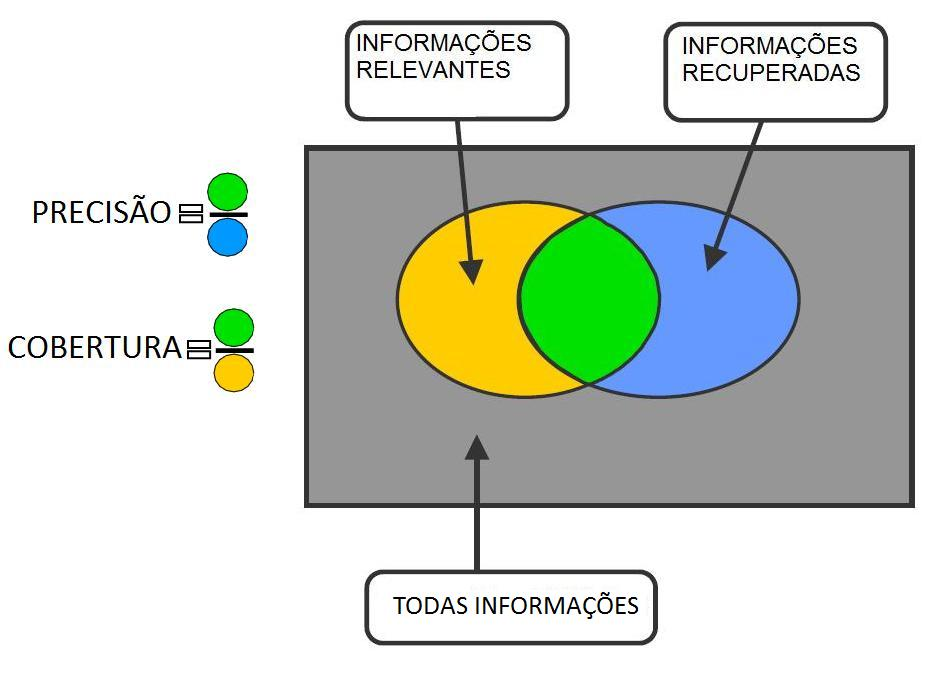
\includegraphics[scale=0.4]{./figuras/avaliacao01.jpg}
				\end{center}				
			\end{figure}
	\end{frame}
	\section{Web Mining}

	\begin{frame}
		\large
		\frametitle{\huge Web Mining}
		\framesubtitle{\Large O que �?}
		\begin{itemize}
			\item \textit{Web Mining} � o uso das t�cnicas de Minera��o de Dados para descobrir e extrair automaticamente a informa��o de documentos na \emph{Web}.% \cite{Etzione1996}.
				
		\end{itemize}				
	\end{frame}
	
	\begin{frame}
		\frametitle{\huge Web Mining}
		\framesubtitle{\Large Minera��o de Dados}		
		\begin{itemize}			
			\item A Minera��o de Dados refere-se ao processo n�o trivial de identifica��o de padr�es v�lidos, previamente desconhecidos e potencialmente �teis de dados.% \cite{Frawley1992}. 				
		\end{itemize}				
	\end{frame}
	
	\begin{frame}
		\frametitle{\huge Web Mining}
		\framesubtitle{\Large KDD - Knowledge Discovery Database}				
		\begin{itemize}						
			\item Seguindo o conceito de Etzione, que utiliza da Descoberta do Conhecimento (\textit{KDD - Knowledge Discovery Database}) como base, ele decomp�e a Web Mining em quatro tarefas: 
			\begin{itemize}
			  \item \emph{Resource finding} (Coleta de Documentos)
			  \item \emph{Information selection and pre-processing} (Pr�-processamento)
			  \item \emph{Generalization} (Extra��o de Padr�es)
			  \item \emph{Analysis} (An�lise)  			  
			\end{itemize}			
		\end{itemize}				
	\end{frame}
	
	\begin{frame}
		\frametitle{\huge Web Mining}
		\framesubtitle{\Large KDD - Knowledge Discovery Database}
		 	\begin{figure}[htb]
				\begin{center}				
					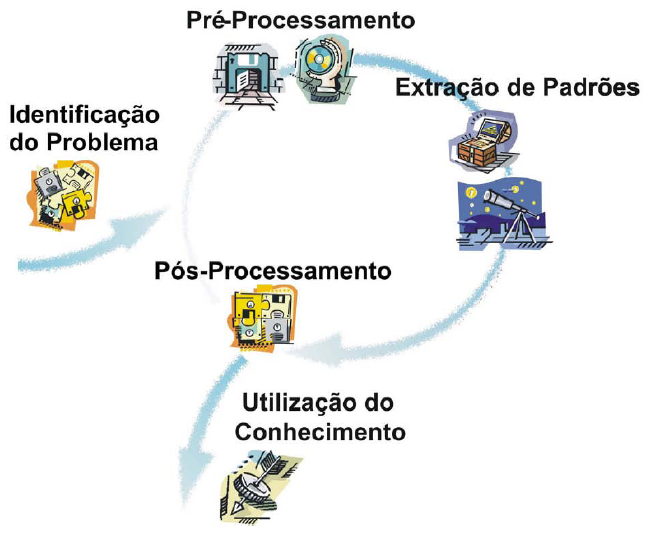
\includegraphics[scale=0.4]{./figuras/processo-kdd.png}
				\end{center}				
	            \label{fig:WM-KDD}
			\end{figure}		
	\end{frame}
	
	\begin{frame}
		\frametitle{\huge Web Mining}				
		 	\begin{figure}[htb]
				\begin{center}				
					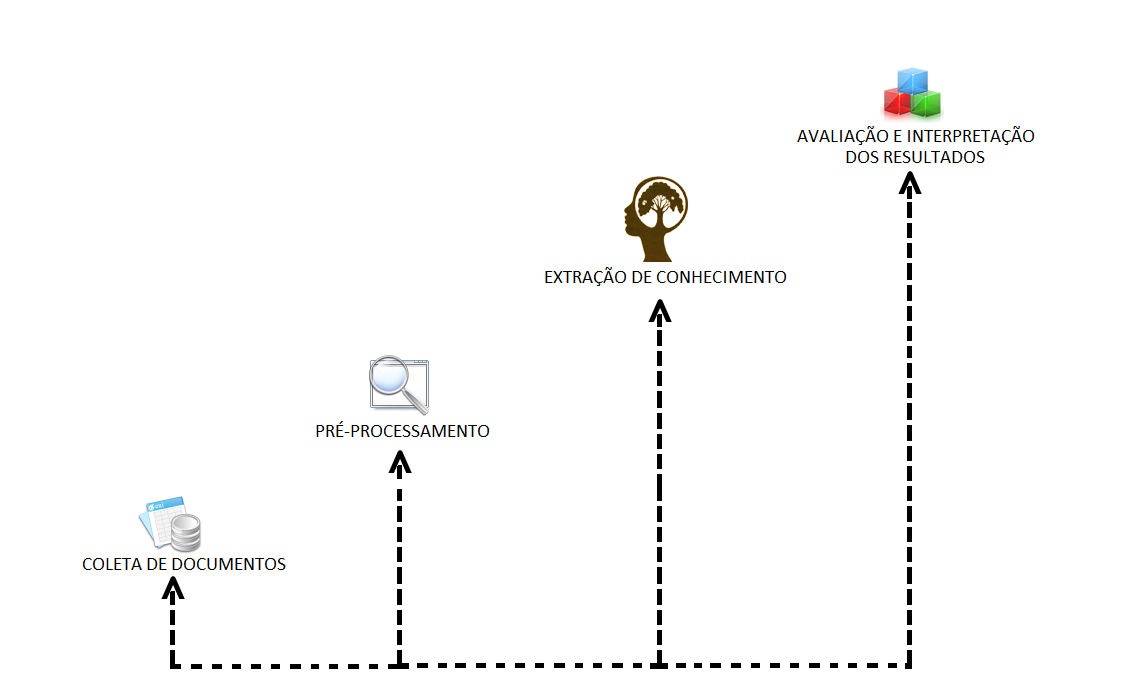
\includegraphics[scale=0.37]{./figuras/processo_webmining.png}
				\end{center}				
	            \label{fig:WM-KDD}
			\end{figure}		
	\end{frame}
	
	\begin{frame}
		\frametitle{\huge Web Mining}
		\framesubtitle{\Large Categorias}
		 	\begin{figure}[htb]
				\begin{center}				
					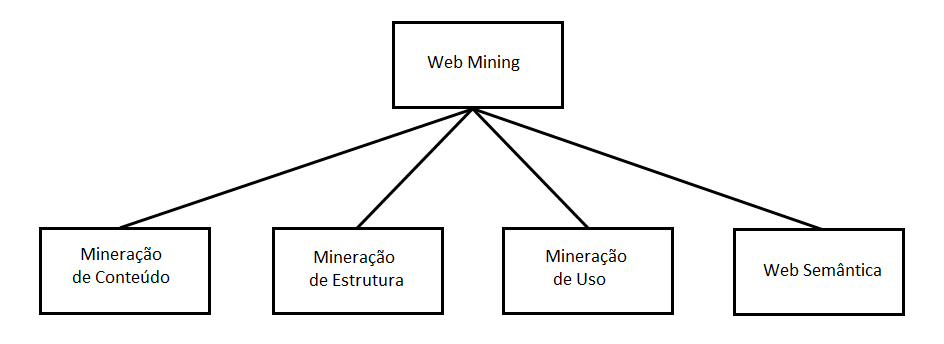
\includegraphics[scale=0.4]{./figuras/WB-taxonomia.png}
				\end{center}				
	            \label{fig:WM-KDD}
			\end{figure}		
	\end{frame}
	
	\section{Conclus\~oes e Trabalhos Futuros}
		
	\begin{frame}
	 	\frametitle{Projeto de Pesquisa Cyted-Salus}
	 	\Large	 	
	 	\center
	 	\begin{block}{Edital CYTED 2006 Redes Tem�ticas}	 	
	 		\begin{itemize}
	 		  \justifying
	 		  \item Avalia��o da qualidade de Sites na �rea da sa�de: uma abordagem baseada em ontologia e minera��o de dados na Web;
	 		  \item Instituto de Inform�tica da Universidade Federal do Rio Grande do Sul; 		   	 		  \item CnPQ / CYTED (Ciencia Y Tecnologia para El Desarrollo).
	 		\end{itemize}									
	 	\end{block}		
	\end{frame}

%Edital CYTED 2006 Redes Tem�ticas -

%Avalia��o da qualidade de Sites na �rea da sa�de: uma abordagem baseada em ontologia e minera��o de dados na Web

%Instituto de Inform�tica da Universidade Federal do Rio Grande do Sul
   
	\begin{frame}	
	 	\frametitle{\huge Conclus\~oes}
		\begin{itemize}
		  \justifying
		 	\item Recupera��o de Informa��o, tomando a \emph{Web} como uma cole��o de documentos, temos um um cen�rio ca�tico quanto a organiza��o e estrutura��o documental. 
			\item Extra��o de Informa��o faz uso das informa��es contidas dos documentos extra�dos para que a informa��o retornada seja um reflexo das necessidades do usu�rio.
			\item \emph{Web Mining}, � a utiliza��o das t�cnicas de Minera��o de Dados cl�ssica contemplando os documentos da \emph{Web} buscando descobrir e extrair padr�es automaticamente, com abordagens que se diferenciam de acordo com o foco estrutural ou de conte�do.
			\item A revolu��o da pr�pria \emph{Web}, nos introduzindo a \emph{Web} Sem�ntica. Com um paradigma de intera��o entre usu�rio e \emph{Web} completamente novo.
		\end{itemize}
	\end{frame}

%	\begin{frame}
%	 	\frametitle{Trabalhos Futuros}
%		\begin{itemize}
%			\item Melhorar a ferramenta de extra��o;			
%		\end{itemize}
%	\end{frame}

	
	%\section{Refer\^encias Bibliogr\'aficas}
	%\bibliographystyle{abnt-alf}
	%\bibliography{./bibliografia/bibliografia}

\end{document}
